% !TEX encoding = UTF-8 Unicode
% !TEX TS-program = xelatex 
\begin{QUESTIONS}
    \begin{QUESTION}
        \begin{ExamInfo}{106}{學測}{單選}{1}
        \end{ExamInfo}
        \begin{QBODY}
            已知某校老師玩過「寶可夢」的比率為${{r}_{1}}$,而學生玩過的比率為${{r}_{2}}$,其中${{r}_{1}}\ne {{r}_{2}}$。
        由下列選項中的資訊,請選出可以判定全校師生玩過「寶可夢」的比率之選項。
        \begin{QOPS}
            \QOP 全校老師與學生比率     
            \QOP 全校老師人數
            \QOP 全校學生人數
            \QOP 全校師生人數
            \QOP 全校師生玩過「寶可夢」人數
        \end{QOPS}
        \end{QBODY}
        \begin{QFROMS}
        \end{QFROMS}
        \begin{QTAGS}
        \end{QTAGS}
        \begin{QANS}
            (1)
        \end{QANS}
        \begin{QSOL}
        \end{QSOL}
        \begin{QEMPTYSPACE}
        \end{QEMPTYSPACE}
    \end{QUESTION}
    \begin{QUESTION}
        \begin{ExamInfo}{106}{學測}{單選}{2}
        \end{ExamInfo}
        \begin{QBODY}
            某個手機程式,每次點擊螢幕上的數$a$後,螢幕上的數會變成${{a}^{2}}$。當一開始時螢幕上的數$b$為正且連續點擊螢幕三次後,螢幕上的數接近${{81}^{3}}$。試問實數$b$最接近下列哪一個選項?
        \begin{QOPS}
            \QOP $1.7$      
            \QOP $3$      
            \QOP $5.2$      
            \QOP $9$      
            \QOP $81$
        \end{QOPS}
        \end{QBODY}
        \begin{QFROMS}
        \end{QFROMS}
        \begin{QTAGS}
        \end{QTAGS}
        \begin{QANS}
            (3)
        \end{QANS}
        \begin{QSOL}
        \end{QSOL}
        \begin{QEMPTYSPACE}
        \end{QEMPTYSPACE}
    \end{QUESTION}
    \begin{QUESTION}
        \begin{ExamInfo}{106}{學測}{單選}{3}
        \end{ExamInfo}
        \begin{QBODY}
            設$\Gamma :\frac{{{y}^{2}}}{{{a}^{2}}}-\frac{{{x}^{2}}}{{{b}^{2}}}=1$為坐標平面上一雙曲線,且其通過第一象限的漸近線為$\ell $。考慮動點$(t,{{t}^{2}})$,從時間$t=0$時出發。當$t>0$時,請選出正確的選項。
        \begin{QOPS}
        \QOP 此動點不會碰到$\Gamma $,也不會碰到$\ell $
        \QOP 此動點會碰到$\Gamma $,但不會碰到$\ell $
        \QOP 此動點會碰到$\ell $,但不會碰到$\Gamma $
        \QOP 此動點會先碰到$\Gamma $,再碰到$\ell $
        \QOP 此動點會先碰到$\ell $,再碰到$\Gamma $
        \end{QOPS}
        \end{QBODY}
        \begin{QFROMS}
        \end{QFROMS}
        \begin{QTAGS}
        \end{QTAGS}
        \begin{QANS}
            (5)
        \end{QANS}
        \begin{QSOL}
        \end{QSOL}
        \begin{QEMPTYSPACE}
        \end{QEMPTYSPACE}
    \end{QUESTION}
    \begin{QUESTION}
        \begin{ExamInfo}{106}{學測}{單選}{4}
        \end{ExamInfo}
        \begin{QBODY}
            在右下圖的正立方體上有兩質點分別自頂點$A,C$同時出發,各自以等速直線運動分別向頂點$B,D$前進,且在1秒後分別同時到達$B,D$。請選出這段時間兩質點距離關係的正確選項。
        
        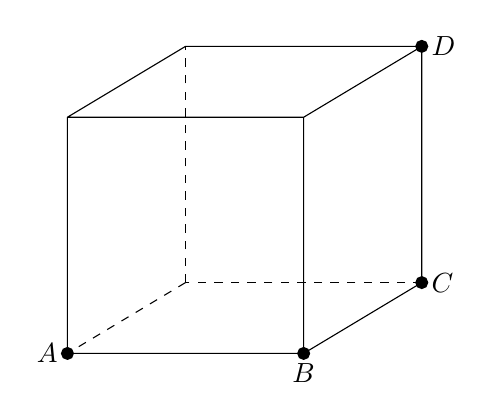
\begin{tikzpicture}[every edge quotes/.append style={auto, text=blue},
        x={(-0.25cm,-0.15cm)},
        y={(0.5cm,0cm)},
        z={(0cm,0.5cm)}]
        %%空間坐標中的CUBE 是以平面上的x軸 y軸再去擴充出深度z軸 z 往前為正,向後為負
        \coordinate (O) at (0,0,0);
        \coordinate (x) at (7,0,0);
        \coordinate (y) at 
        (0,7,0);
        \coordinate (z) at (0,0,7);
        
        \coordinate (Base1) at (0,0,0);
        \coordinate (Base2) at (6,0,0);
        \coordinate (Base3) at (6,6,0);
        \coordinate (Base4) at (0,6,0);
        \coordinate (Base1Up) at (0,0,6);
        \coordinate (Base2Up) at (6,0,6);
        \coordinate (Base3Up) at (6,6,6);
        \coordinate (Base4Up) at (0,6,6);
        
        \coordinate (A) at (Base2);
        \coordinate (B) at (Base3);
        \coordinate (C) at (Base4);
        \coordinate (D) at (Base4Up);
        
        \draw [draw=black, every edge/.append style={draw=black, dashed}]
        (Base1) edge (Base2)
        (Base2) -- (Base3)
        (Base3) -- (Base4)
        (Base4) edge (Base1)
        (Base1Up) -- (Base2Up)
        (Base2Up) -- (Base3Up)
        (Base3Up) -- (Base4Up)
        (Base4Up) -- (Base1Up)
        (Base1) edge (Base1Up)
        (Base2) -- (Base2Up)
        (Base3) -- (Base3Up)
        (Base4) -- (Base4Up);
        
        \foreach \v/\u/\t in 
        { A/left/$A$,
            B/below/$B$,
            C/right/$C$,
            D/right/$D$
        }
        {
            \draw[ultra thick,fill] (\v) circle (1.5pt);
            \node[\u] at (\v){\t};
        }; 
        
        \end{tikzpicture}
        
        \begin{QOPS}
            \QOP 兩質點的距離固定不變
            \QOP 兩質點的距離越來越小
            \QOP 兩質點的距離越來越大
            \QOP 在$\frac{1}{2}$秒時兩質點的距離最小
            \QOP 在$\frac{1}{2}$秒時兩質點的距離最大
        \end{QOPS}
        \end{QBODY}
        \begin{QFROMS}
        \end{QFROMS}
        \begin{QTAGS}
        \end{QTAGS}
        \begin{QANS}
            (4)
        \end{QANS}
        \begin{QSOL}
        \end{QSOL}
        \begin{QEMPTYSPACE}
        \end{QEMPTYSPACE}
    \end{QUESTION}
    \begin{QUESTION}
        \begin{ExamInfo}{106}{學測}{單選}{5}
        \end{ExamInfo}
        \begin{QBODY}
            下圖是某城市在2016年的各月最低溫(橫軸$x$)與最高溫(縱軸$y$)的散佈圖。
        
        今以溫差(最高溫減最低溫)為橫軸且最高溫為縱軸重新繪製一散佈圖。試依此選出正確的選項。
        \begin{QOPS}
            \QOP 最高溫與溫差為正相關,且它們的相關性比最高溫與最低溫的相關性強
            \QOP 最高溫與溫差為正相關,且它們的相關性比最高溫與最低溫的相關性弱
            \QOP 最高溫與溫差為負相關,且它們的相關性比最高溫與最低溫的相關性強
            \QOP 最高溫與溫差為負相關,且它們的相關性比最高溫與最低溫的相關性弱
            \QOP 最高溫與溫差為零相關
        \end{QOPS}
        \end{QBODY}
        \begin{QFROMS}
        \end{QFROMS}
        \begin{QTAGS}
        \end{QTAGS}
        \begin{QANS}
            (4)
        \end{QANS}
        \begin{QSOL}
        \end{QSOL}
        \begin{QEMPTYSPACE}
        \end{QEMPTYSPACE}
    \end{QUESTION}
    \begin{QUESTION}
        \begin{ExamInfo}{106}{學測}{單選}{6}
        \end{ExamInfo}
        \begin{QBODY}
            試問有多少個實數$x$滿足$\frac{\pi }{2}\le x\le \frac{3\pi }{2}$且$\cos x{}^\circ \le \cos x$?
        \begin{QOPS}
            \QOP $0$個     
            \QOP $1$個     
            \QOP $2$個     
            \QOP $4$個     
            \QOP 無窮多個
        \end{QOPS}
        \end{QBODY}
        \begin{QFROMS}
        \end{QFROMS}
        \begin{QTAGS}
        \end{QTAGS}
        \begin{QANS}
        \end{QANS}
        \begin{QSOL}
        \end{QSOL}
        \begin{QEMPTYSPACE}
        \end{QEMPTYSPACE}
    \end{QUESTION}
    \begin{QUESTION}
        \begin{ExamInfo}{106}{學測}{單選}{7}
        \end{ExamInfo}
        \begin{QBODY}
            小明想要安排從星期一到星期五共五天的午餐計畫。他的餐點共有四種選擇:牛肉麵、大滷麵、咖哩飯及排骨飯。小明想要依據下列兩原則來安排他的午餐:
        (甲)每天只選一種餐點但這五天中每一種餐點至少各點一次
        (乙)連續兩天的餐點不能重複且不連續兩天吃麵食
        根據上述原則,小明這五天共有幾種不同的午餐計畫?
        \begin{QOPS}
            \QOP $52$      
            \QOP $60$      
            \QOP $68$      
            \QOP $76$      
            \QOP $84$
        \end{QOPS}
        \end{QBODY}
        \begin{QFROMS}
        \end{QFROMS}
        \begin{QTAGS}
        \end{QTAGS}
        \begin{QANS}
            (2)
        \end{QANS}
        \begin{QSOL}
        \end{QSOL}
        \begin{QEMPTYSPACE}
        \end{QEMPTYSPACE}
    \end{QUESTION}

\end{QUESTIONS}